\chapter{Preliminary experiments} \label{ch:baseline}

We will first perform some experiments using some simple models. These will
both serve as demonstrations that learning is feasible, and as baselines to
which we will compare results using more complex models. In addition, we are
comparing the performance of different kinds of input. We use both tokens,
character \ngrams, mixed POS and function word \ngrams, and \ac{POS} \ngrams
as inputs.

We will compare nominal classification, ordinal regression and numeric
regression as different formulations of the \ac{AES} task, and see which
performs best. We will also investigate different evaluation metrics for the
task.


\section{Preprocessing}

The data files in the ASK corpus are in \ac{XML} format, and contain
information about tags, mistakes and corrections, paragraphs, sentences and
more. These files were transformed into several other formats during
preprocessing. First, they were converted to plain text files, stripped of
all tags or correction labels. The text files have one sentence per line,
consisting of space-separated tokens, and an empty line separating
paragraphs.

These raw text files were then sent through the text processing pipeline
UDPipe \autocite{udpipe:2017} for tagging and dependency parsing. The UDPipe
project maintains an online REST \ac{API} containing a selection of
pre-trained models. All documents were transformed by the REST \ac{API} using
what was at the time of writing the newest Norwegian bokmål (nb) model
available\footnote{\texttt{norwegian-bokmaal-ud-2.3-181115}}.

The pipeline accepts different input formats, including raw text files on
this format. We used the tokenization from the ASK corpus and not the
tokenization algorithm built into UDPipe. The output from UDPipe is on the
CoNLL file format, with a single token per line. UDPipe tags the documents
using the Universal Dependencies (UD) tagset, referred to as UPOS. The
original tags in the ASK corpus are from the Oslo-Bergen tagger's own tagset
\autocite{oslobergen}, and these were not used in any of our experiments.


\section{Metrics} \label{sec:metrics}

For each class, we can compute the \emph{precision} and \emph{recall} (Eq.
\ref{eq:precision}). The precision for a class is the ratio of examples that
were predicted to belong to the class which actually belong to the class. The
recall for a class is the ration of examples that actually belong to the
class which were predicted to belong to the class. The \FI score for a class
is the harmonic mean of the precision and recall . It can also be expressed
directly as a function of the number of true positives ($TP$), false
negatives ($FN$), and false positives ($FP$), as in equation \ref{eq:fscore}.

\begin{gather}
  \begin{aligned}\label{eq:precision}
    precision = \frac{TP}{TP + FP} \qquad recall = \frac{TP}{TP + FN}
  \end{aligned}
  \\[2ex]
  F_1 = 2\cdot\frac{precision\cdot recall}{precision+recall}
      = {\frac{2\cdot TP}{2\cdot TP + FN + FP}}\label{eq:fscore}
\end{gather}

In a multi-class prediction setup, there are several ways to combine the
classes' individual \FI scores into a single metric. There is the micro
average \FI, which is equal to accuracy in the case where all samples have
exactly one true label. Since this is the case for our data, we will
sometimes refer to micro \FI or accuracy interchangeably. Accuracy is the
proportion of samples where the gold labels and predicted labels are the
same.

Then there is the macro average, which is the unweighted average of \FI
scores for all classes. When the distribution of classes is uneven, a macro
average will give proportionally more weight on samples from small classes,
and less weight to all samples in classes with large support. A model with a
high micro \FI and a low macro \FI indicates that it is good at classifying
examples from the most frequent classes, but performs worse on classes with
low support.

In addition to macro and micro average, the weighted \FI is a weighted
average where each class is weighted proportionally to its share of the
complete dataset.

\FI scores previously reported in \ac{AES} literature include Micro \FI score
in \textcite{vajjala17}, and weighted \FI in
\textcite{vajjala18universalCEFR}. For the \ac{NLI} task, micro \FI is
reported in \textcite{malmasi15,malmasi17}. \FI score is also reported in
\textcite{hancke2013,pilan2016}. We find it safe to assume that the \FI in
these two studies refer to the macro average \FI, even though they are not
explicit about whether it is the case. In \textcite{vajjalaloo2014}, \FI
scores are reported separately for each class.

Other, non-\FI metrics that have been reported in \ac{AES} literature include
\ac{QWK} \autocite{taghipour16, alikaniotis2016automatic}, Pearson's
correlation coefficient \autocite{vajjala17, alikaniotis2016automatic},
Spearman's rank correlation coefficient and root mean squared error
\autocite{alikaniotis2016automatic}, and mean absolute error
\autocite{vajjala17}. These are metrics that may depend on the ordinal nature
of proficiency scores, and potentially the relative differences between
different scores. For instance, a prediction of `C1' for an essay with gold
label `B1' is a more serious misclassification than a prediction of `A2/B1'
for the same sample, and this can be taken into account by some metrics.

According to \textcite{yannakoudakis2015evaluating}, there are several
problems with using \ac{QWK} as a metric for the \ac{AES} task. The metric
depends on trait prevalence, the scoring scale and the marginal distributions
of labels and predictions, among other issues. Therefore it is problematic to
compare \ac{QWK} scores between different systems and datasets. However,
since two of the cited studies are based on a dataset from a Kaggle
competition where \ac{QWK} was the official metric, the authors of the
studies have chosen to report this metric, either alone or in conjunction
with other metrics.


\subsection{Reported metrics}

Two different sets of output labels are used in our experiments: The original
seven CEFR labels, and a collapsed set where the intermediate classes, such
as ``A2/B1'', are rounded up to the nearest canonical class, i.e. the CEFR
label after the slash. This results in only four different labels: ``A2'',
``B1'', ``B2'' and ``C1''. We will focus on comparing the models based on
their performance on the full set of labels, but include the performance on
collapsed labels because the setup is more similar to other \ac{AES} studies
using different datasets using CEFR labels without intermediate classes.

We run two parallel experiments for each model. One where we train and
evaluate on the full set of classes, and one where we train and evaluate on
the collapsed classes. We report both the macro and micro \FI for both modes.

A third option, namely to train on the full set of classes and reduce the
predictions to the collapsed set of classes, was also attempted, based on the
assumption that the more fine grained labels in the full set of classes can
provide useful supervision signals even though we evaluate on a smaller set.
However, in practice we observed that the best performing models on the
collapsed labels were the models that were also trained on the collapsed
tags. Therefore, we do not report any results from this evaluation mode.


\section{Model descriptions}

Initial experiments were run using linear models, logistic regression,
and linear regression, and neural models following the \acp{MLP} architecture.


\subsection{Classification versus regression}

\ac{AES} can be modelled both as a classification task and as a regression
task, and both are seen in previous work. Sometimes both have used in the
same study. For instance, in \textcite{vajjala17}, two different datasets
with different properties were used, and the author utilized both multi-class
prediction and regression at different points.

A problem with using regression for the AES task is, in theory, that while we
know the ordering of proficiency classes, we do not know the distance between
adjacent classes. For instance, we cannot know if the jump from CEFR score
`A2/B1' to 'B1' is just as big as `B1' to `B1/B2'. However, we need to
implicitly decide this when we transform the labels into numeric values for
regression. In practice we place the classes with equal distance over a
numeric interval.

This challenge of quantifying distance between classes does not apply to the
classification approach, but it comes with another problem. Multi-class
classification does not consider any ordering of classes, which is an
intrinsic property of the classes for AES. However, we do not have to make
assumptions about the distance between classes.

A third class of analysis called \emph{ordinal regression} or \emph{ranking
learning} is intended for predicting an ordinal variable, where classes are
distinct, but have a natural ordering. In theory, it is the most fitting
formulation for the \ac{AES} task with nominal classes, since we know the
ordering of the classes, but not the distance between them. However, unlike
regression and nominal classification, algorithms for ordinal regression are
implemented in common machine learning frameworks like scikit-learn. We will
however explore a formulation of ordinal regression for a neural model, as
described in section \ref{subsec:ordreg}.


\subsection{Input representations}

Input representations are shared between the linear and neural models, except
for the total number of features. The neural models may restrict the number
of features by cutting off less frequently occurring features, and this is
noted below.

\subsubsection*{Word counts}

This representation is a vector with a entry for each unique word form in the
training data, 20,766 in total. The value of each entry is the number of
times the word form occurs in the document. The neural models limits the
count vectors to the 10,000 most common tokens.

\subsubsection*{Character \ngrams}

Documents are represented by count vectors where each entry represents a
\ngram of characters. Some examples of character \ngrams are
$\langle$eg␣$\rangle$, $\langle$␣i␣$\rangle$ or $\langle$si$\rangle$. For the
linear model, all \ngrams with $n\in \{1,2,3\}$ were used, and for the neural
models the 10,000 most commonly occurring \ngrams with $n\in \{2,3,4\}$ were
used.

\subsubsection*{POS \ngrams}

Documents are represented by count vectors where each entry represents a
\ngram of POS tags. Some examples of POS \ngrams are $\langle$NOUN
NOUN$\rangle$, $\langle$PRON AUX PRON$\rangle$ or $\langle$SCONJ
ADJ$\rangle$. For the linear model, all \ngrams with $n\in \{1,2,3\}$ were
used, and for the neural models the 10,000 most commonly occurring \ngrams
with $n\in \{2,3,4\}$ were used.

\subsubsection*{Mixed POS}

The Mixed POS mode was taken from \textcite{malmasi15}. Their best performing
single feature was a mix of word forms and POS tags, so that common function
words appeared in their written form, while content words were substituted
with their POS tag. We used the same set of function words as
\citeauthor{malmasi15}.

\begin{example}
% cSpell:disable-next
\gll generasjoner kan også få   anledning til å utnytte dem  
% cSpell:disable-next
     NOUN         kan også VERB NOUN      til å VERB    dem  
\glt `generations can also have the opportunity to exploit them'
\glend
\label{ex:mixed-pos}
\end{example}

Example \ref{ex:mixed-pos} shows a sentence fragment with the original series
of tokens, the sequence of mixed function words and UPOS tags it is
transformed into, as well as a translation into English.

The \ngram features add a certain sensitivity to local order of features.
Many character \ngrams will represent entities smaller than a word, but may
indicate common spelling mistakes. \ac{POS} and Mixed POS \ngrams, on the
other hand, might be able to represent syntactic features. Spelling and
syntax should be correlated with L2 proficiency, and traditional \ac{ML}
methods that rely on manual feature engineering have included domain specific
features designed to capture spelling and syntax, as for instance in
\textcite{vajjala17}.

We used the same set of stop words as \citeauthor{malmasi15}. From these
transformed sequences, we extracted \ngrams in the interval $[1,3]$. The
20,000 most commonly occurring of these were used for the neural models.


\subsection{Linear models} \label{subsec:linear}

The purpose of linear models in the context of this thesis is to establish
baseline results, and investigate the performance of regression versus
nominal classification for the task. Since the main goal of the thesis is to
investigate neural models, we have not spent any effort tuning
hyperparameters for the linear models, and instead kept the default
parameters from the library implementation.

The logistic regression model was implemented using the Python library
scikit-learn \autocite{scikit-learn}. The model was instantiated with the
`lgbfs' solver to minimize multinomial loss. This solver was chosen because
it is set to become the default solver in a future version of scikit-learn.
No regularization was used, and the optimizer was set to run for a maximum of
100 iterations.

The linear regression model was a support vector regressor also chosen from
scikit-learn. The default parameters were used, which are epsilon-insensitive
loss with $\epsilon=0$, a penalty parameter of $1$, and a tolerance of
$10^{-4}$ for the stopping criteria.

In order to report classification based metrics for a regression model, we
had to transform the predicted scores, which are continuous, into discrete
scores equivalent to the given classes. This was by rounding the raw
regression scores to the nearest integer. The output from the support vector
regression model is not constrained to any interval, making it necessary to
additionally clip the output values to the range of scores: $[0,6]$ in our
full set of labels and $[0,3]$ in the collapsed set.


\subsection{Multi-layer perceptron} \label{subsec:mlp}

The MLP models were implementing in Keras \autocite{keras} and run on the
TensorFlow backend \autocite{tensorflow}. All the models the have an input
layer with 20,000 dimensions, followed by two fully connected layers with 100
and 300 nodes, respectively. The fully connected layers use \ac{ReLU}
activation and dropout regularization with a dropout rate of 50\%.

The output layer varies depending on the method used. For multi-class
prediction, we use an output layer with softmax activation and 7 or 4
dimensions, depending on whether we run with collapsed labels or not. The
multi-class model was trained by minimizing the categorical cross-entropy
loss (Eq. \ref{eq:crossentropy}).

For regression, our output layer contains a single node with sigmoid
activation. The regression model is trained by minimizing the mean squared
error loss against gold labels normalized to the interval $[0, 1]$.
Normalization is a scaling operation such that the lowest class maps to 0,
the highest class to 1, and all classes are evenly spaced. This is in line
with the method for neural network regression used by \textcite{taghipour16}.
For evaluating the predictions, the output is scaled back using the value of
the highest label and transformed into categorical values using the method
described in subsection \ref{subsec:linear}. This means that with $C$ classes,
we actually scale by $C-1$, such that 0 maps directly to the lowest class and
1 directly to the highest.

Because the sigmoid function is non-linear, values that are evenly spaced in
its output domain are not evenly spaced in the input. The sigmoid function is
steepest in the region around zero, where its value is close to $0.5$. A
consequence of this is that when we map the classes to the range of the
sigmoid function, the central classes correspond to a smaller set of input
values than the peripheral classes. In fact, the lowest and highest classes
correspond to an unbounded set of input values. Regardless, we will see that
the classes which the model struggles the most to predict correctly are the
peripheral classes.

\subsubsection{Ordinal regression} \label{subsec:ordreg}

For ordinal regression, we implemented a neural model for ordinal regression
following a modified version of the method in \textcite{cheng2008neural}.
Gold labels are represented as a vectors of size $C-1$ where the elements are
filled with ones from left to right such that: The lowest class is all zeros.
The next class is a single one in the leftmost position and zeros in the
remaining positions. The next class has two ones in the two leftmost
positions, continuing to the highest class which is represented by a vector
of only ones.

In the original paper, \citeauthor{cheng2008neural} used vectors of size $C$,
and mapped the lowest class to a where the first element was one. The authors
did not use an all-zero vector as a gold label at all, but at test time would
assign an all-zero vector to the lowest class.

Our formulation only uses $C-1$ elements to represent the thresholds between
classes. This approach for ordinal regression with neural models is one of
several that are described in a survey paper for ordinal regression
\autocite{gutierrez2016ordinal}. The authors of the survey describe several
binary decomposition methods for ordinal regression problems, and our
approach is the same as they call \emph{Ordered Partitions}.

The output layer of our neural network has size $C-1$ and uses element-wise
sigmoid activation to constrain the values of elements to the interval
$(0,1)$. At train time, we minimize the mean square error between the gold
labels and output.

At predict time, we convert the sigmoid activated values to either ones or
zeros by comparing them to a threshold, in our case $0.5$. The resulting
vector may be any sequence of ones and zeros, even those not conforming to
our rule for representing classes, i.e. there might be a one to the right of
a zero. We then select the predicted class by taking the index of the first
zero element of this vector, or the highest class if all elements are one. In
this way, assuming a total of four different classes, $[0,0,0]$ and $[0,0,1]$
are both assigned to the lowest class, since the first element is zero.
$[1,1,0]$ is the only vector that is assigned to the second-highest class,
and $[1,1,1]$ is the only vector assigned to the highest class.

The multi-class and ordinal regression neural networks were trained using the
Adam optimization algorithm \autocite{kingma2014adam} with a learning rate of
$2\cdot 10^{-4}$. The neural regressor was trained with the RMSProp
optimization algorithm using the default learning rate of $10^{-3}$.


\subsection{Controlling randomness}

We took several measures to ensure reproducible results from our experiments.
One was to fix the seeds to the random seeds in Python and associated libraries
used for the experiments. Since the software uses pseudo-random generators,
the same seed will always yield the same sequence of numbers when a program
is run again. In addition to the random number generators, Python can use a
configured seed value to compute hashes of strings and other values. Without a
way to control the Python hash seed, the mapping of e.g. word tokens to indices
would be different on each run.

Second, we disabled parallel execution in the computation graphs underlying
the neural models. Parallel execution is a source of non-determinism, because
there is no guarantee that sub-computations will always finish in the same order,
and because floating point numbers have limited precision, adding the same
numbers in a different order can give small rounding errors which can compound
over time.


\section{Results}

All macro and micro \FI scores for the classifiers described in this chapter,
for both the full and collapsed sets of classes, are found in table
\ref{tab:baseline-accuracies}.

\begin{table}
  \centering
  \begin{tabular}{lrrrr}
    \toprule
             & \multicolumn{2}{c}{All labels} & \multicolumn{2}{c}{Collapsed labels} \\
    \cmidrule(lr){2-3}
    \cmidrule(lr){4-5}
    Model      & Macro \FI & Micro \FI & Macro \FI & Micro \FI \\
    \midrule
    Majority   &  $0.040$  &  $0.163$  &  $0.127$  &  $0.341$ \\
    \midrule
    % $BEGIN autotable baseline-accuracies
    % $META models-per-row=2 columns-per-model=macrof1,microf1
    % $ROW LogReg BOW: linear_logreg-1337_1 linear_logreg-1338_1
    % $ROW LogReg Char: linear_logreg-1337_2 linear_logreg-1338_2
    % $ROW LogReg POS: linear_logreg-1337_3 linear_logreg-1338_3
    % $ROW LogReg Mix: linear_logreg-1337_4 linear_logreg-1338_4
    % \midrule
    % $ROW SVC BOW: linear_svc-1337_5 linear_svc-1338_5
    % $ROW SVC Char: linear_svc-1337_6 linear_svc-1338_6
    % $ROW SVC POS: linear_svc-1337_7 linear_svc-1338_7
    % $ROW SVC Mix: linear_svc-1337_8 linear_svc-1338_8
    % \midrule
    % $ROW SVR BOW: linear_svr-1337_9 linear_svr-1338_9
    % $ROW SVR Char: linear_svr-1337_10 linear_svr-1338_10
    % $ROW SVR POS: linear_svr-1337_11 linear_svr-1338_11
    % $ROW SVR Mix: linear_svr-1337_12 linear_svr-1338_12
    % \midrule
    % $ROW MLP BOW:    mlp_bow-26436597_13 mlp_bow-26436607_13
    % $ROW MLP Char:   mlp_char-26436597_14 mlp_char-26436607_14
    % $ROW MLP POS:    mlp_pos-26436597_15 mlp_pos-26436607_15
    % $ROW MLP Mix:    mlp_mix-26436597_16 mlp_mix-26436607_16
    % \midrule
    % $ROW MLP Reg BOW:    mlp_bow-26436597_17  mlp_bow-26436607_17
    % $ROW MLP Reg Char:   mlp_char-26436597_18 mlp_char-26436607_18
    % $ROW MLP Reg POS:    mlp_pos-26436597_19  mlp_pos-26436607_19
    % $ROW MLP Reg Mix:    mlp_mix-26436597_20  mlp_mix-26436607_20
    % \midrule
    % $ROW MLP Rank BOW:   mlp_bow-26449272_21  mlp_bow-26449273_21
    % $ROW MLP Rank Char:  mlp_char-26449272_22 mlp_char-26449273_22
    % $ROW MLP Rank POS:   mlp_pos-26449272_23  mlp_pos-26449273_23
    % $ROW MLP Rank Mix:   mlp_mix-26449272_24  mlp_mix-26449273_24
    % $END autotable
    LogReg BOW & $0.199$ & $0.317$ & $0.384$ & $0.626$ \\
    LogReg Char & $0.221$ & $0.317$ & $0.399$ & $0.602$ \\
    LogReg POS & $0.190$ & $0.301$ & $0.312$ & $0.569$ \\
    LogReg Mix & $0.213$ & $0.341$ & $0.337$ & $0.577$ \\
    \midrule
    SVC BOW & $0.210$ & $0.317$ & $0.391$ & $0.610$ \\
    SVC Char & $0.189$ & $0.293$ & $0.347$ & $0.537$ \\
    SVC POS & $0.157$ & $0.244$ & $0.336$ & $0.618$ \\
    SVC Mix & $0.215$ & $0.350$ & $0.319$ & $0.585$ \\
    \midrule
    SVR BOW & $\mathbf{0.444}$ & $0.415$ & $0.429$ & $0.659$ \\
    SVR Char & $0.252$ & $0.317$ & $0.440$ & $0.602$ \\
    SVR POS & $0.334$ & $0.358$ & $\mathbf{0.476}$ & $0.593$ \\
    SVR Mix & $0.312$ & $0.350$ & $0.441$ & $0.659$ \\
    \midrule
    MLP BOW & $0.252$ & $0.398$ & $0.382$ & $0.659$ \\
    MLP Char & $0.264$ & $0.415$ & $0.417$ & $0.675$ \\
    MLP POS & $0.237$ & $0.407$ & $0.393$ & $0.642$ \\
    MLP Mix & $0.232$ & $0.398$ & $0.353$ & $0.659$ \\
    \midrule
    MLP Reg BOW & $0.246$ & $0.341$ & $0.458$ & $\mathbf{0.715}$ \\
    MLP Reg Char & $0.286$ & $0.341$ & $0.468$ & $0.707$ \\
    MLP Reg POS & $0.273$ & $0.390$ & $0.418$ & $0.699$ \\
    MLP Reg Mix & $0.252$ & $0.423$ & $0.440$ & $0.650$ \\
    \midrule
    MLP Rank BOW & $0.276$ & $0.398$ & $0.408$ & $0.707$ \\
    MLP Rank Char & $0.330$ & $\mathbf{0.480}$ & $0.395$ & $0.634$ \\
    MLP Rank POS & $0.251$ & $0.382$ & $0.420$ & $0.667$ \\
    MLP Rank Mix & $0.235$ & $0.366$ & $0.403$ & $0.634$ \\
    \bottomrule
  \end{tabular}
  \caption[\FI scores of linear and neural classifiers]{
    \FI scores of various classifiers. LogReg is logistic regression, SVC is
    support vector classification, SVR is support vector regression, MLP is
    multi-layer perceptron. BOW is bag-of-words input, Char is character
    \ngrams, POS is UPOS \ngrams, Mix is mixed UPOS \ngrams.
  }
  \label{tab:baseline-accuracies}
\end{table}

As a simple baseline, we consider the majority class classifier. The majority
class in the training set is ``B1'', both with the full class set of labels
and with the collapsed set. The macro \FI scores for the majority classifier
are very low, as the majority class classifier predicts no samples for any
classes except the majority, and thus the \FI score for all other classes is
zero\footnote{Technically, the precision is undefined when there are no
predictions for the class, but it is commonly set to 0 in this case.}.


\subsection{Linear models}

Moving to a linear model, a logistic regression classifier (LogReg) using
bag-of-words features achieves a macro \FI score of 19.9\% on the dev set
without collapsed labels and 38.4\% with collapsed labels, and thus beats the
majority classifier by a large margin. However, the classifier performs
better using another input representation than bag-of-words. Character
\ngrams yields the highest macro \FI scores using a logistic regression
classifier, 22.1\% and 39.9\% for all classes and collapsed classes,
respectively.

The \ac{SVM} classifier, referred to as SVC in the table, performs around the
same level as the LogReg classifier. Its highest macro \FI scores, 21.5\% and
39.9\%, are lower than for LogReg. The \ac{SVM} regressor, referred to as
SVR, improves on all macro \FI scores from the linear classifiers, and also
has the highest micro \FI scores of all the linear models. Using bag-of-words
input, the model yields a macro \FI of 44.4\% on the full set of labels. For
the collapsed set of labels, the highest macro \FI, 47.6\%, comes from POS
\ngram features.


\subsection{Neural networks}

The \ac{MLP} classifier is referred to in table \ref{tab:baseline-accuracies}
as MLP. The network with a single node regression output is called MLP Reg,
and the ordinal regression model is called MLP Rank.

For all the different input representations, the \ac{MLP} classifier is
outperformed in terms of macro \FI by one or both of the other two neural
models.

In order to examine the classification behaviour closer, we present the
confusion matrices from one of the neural networks trained and evaluated on
the complete set of classes. We chose the MLP model using ordinal regression
and character \ngrams as input (MLP Rank Char), as it had higher accuracy
than any other linear or neural model, as well as the highest macro \FI of
the neural models. Refer to figures \ref{fig:mlp-char-rank} and
\ref{fig:mlp-char-rank-round}.

We want predictions to lie on the diagonal of the matrix. This is true for
all classification tasks. However, due to the ordinal nature of the CEFR
scores, we also want eventual mis-classifications to lie close to the
diagonal, which would indicate a small magnitude of misclassification.
Conversely, we do not want any predictions in the upper right and lower left
corners, as they represent mis-classifications of the greatest magnitude.

What we see is that while the predictions are not perfectly on the diagonal,
they tend to it. For four out of seven rows, and five out of seven columns
(all columns with predictions), the highest value is on the diagonal.
However, despite the tendency toward the diagonal, there are several severe
mis-classifications, such as three `B2/C1' texts being classified as `B1' and
`A2/B1'.

MLP Char Rank has 2,032,206 parameters which are all trainable. For collapsed
labels, the number of parameters is 2,031,303.

\begin{figure}
  % mlp_char-26449272_22 
  \centering
  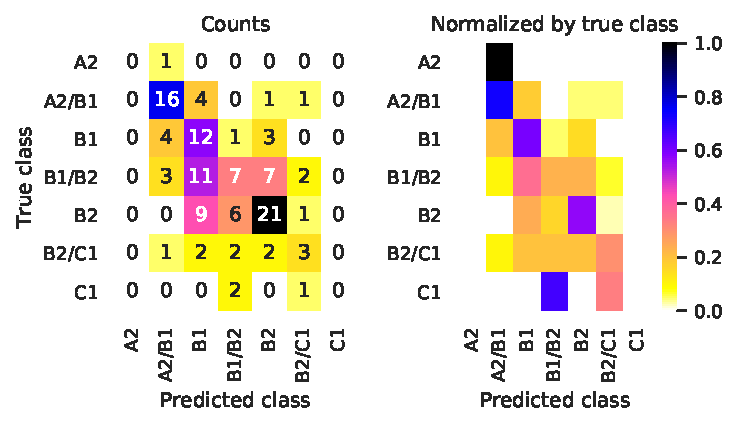
\includegraphics{mlp-char-rank}
  \caption[Confusion matrix for MLP Rank Char]{
    The confusion matrix for a multi-layer perceptron with ordinal regression
    output, using character \ngrams as input.
  }
  \label{fig:mlp-char-rank}
\end{figure}

\begin{figure}
  % mlp_char-26449273_22 
  \centering
  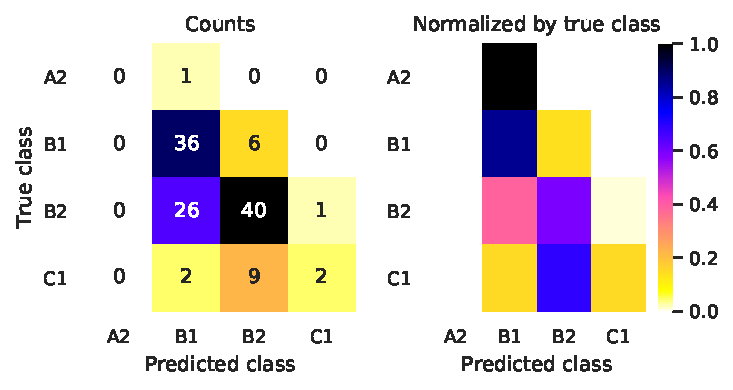
\includegraphics{mlp-char-rank-round}
  \caption[Confusion matrix for MLP Rank Char, collapsed labels]{
    The confusion matrix for a multi-layer perceptron with ordinal regression
    output, using character \ngrams as input. Trained and evaluated using
    collapsed CEFR labels.
  }
  \label{fig:mlp-char-rank-round}
\end{figure}


\section{Conclusion}

We have looked at a number of different evaluation metrics that have
previously been used in the \ac{AES} literature, and decided on macro and
micro \FI scores as the metrics to focus on in this project.

We have explored a selection of different classifier models, both linear and
neural architectures. We have compared three different prediction modes, and
seen that regression and ordinal regression had better performance on the
task than nominal classification.

We have tried out a selection of different input representations for our
systems. We saw that the best input representation is dependent on the model
in question.
